% !TeX root = main.tex
% !TeX program = pdflatex
\documentclass[anon]{opt2026}

\usepackage{booktabs}
\usepackage{microtype}
\usepackage{xcolor}
\usepackage{enumitem}

\title[Deep Unfolding and Failure Modes in Joint Sparse Recovery]
{Deep Unfolding and Failure Modes in Joint Sparse Recovery with Unknown Illumination}

% Hidden by the official class in anonymous mode. Replace only for camera-ready.
\optauthor{\Name{Anonymous Authors} \Email{anonymous@example.com}\\
\addr Anonymous Institution}

\begin{document}
\maketitle

\begin{abstract}
We study a block-coordinate optimizer for compressive imaging when the measured
signal is the product of a sparse scene and an unknown smooth illumination
field.  The coefficient block is a nonsmooth Lasso problem solved by FISTA,
while the illumination block is a regularized least-squares problem.  On five
natural-image patches, joint optimization improves PSNR by up to $4.7$ dB on
textured scenes but loses $7.8$--$10.0$ dB on a low-energy scene.  A natural
conditioning-number gate fails: the worst scene has the \emph{best} measured
conditioning.  Separately, over five optimizer seeds a ten-layer tied LISTA
reaches NMSE $0.0435\mathbin{\pm}0.0120$, which FISTA needs 23 iterations to
match.  This $2.3\times$ iteration reduction does not yield a batch-1 CPU
latency gain at $N=200$ ($0.664$ versus $0.484$ ms).  We characterize both the
scene-energy failure and the poor scaling of the present dense implementation.
The results show that identifiability and operator structure, not iteration
count alone, govern a practical joint optimizer.
\end{abstract}

\section{Introduction}

Optimization-based imaging often separates reconstruction from image-signal
processing.  This ordering is questionable when a nuisance field changes the
very representation on which the reconstruction prior relies.  We consider
measurements
\begin{equation}
  y=A\,\operatorname{diag}(g_{\mathrm{pix}})\Psi c+w,
  \label{eq:forward}
\end{equation}
where $c\in\mathbb{R}^N$ is sparse, $\Psi$ is a two-dimensional DCT synthesis
operator, $g\in\mathbb{R}^{q}$ is a smooth per-column illumination vector with
$q=\sqrt{N}$, and $g_{\mathrm{pix}}$ tiles $g$ over image rows.  Recovering the
illuminated image and correcting it afterwards applies the sparsity prior to
the product rather than the scene.  We instead optimize both variables.
This places the study in classical compressed sensing
\citep{candes2006stable,donoho2006compressed}, with an additional bilinear
nuisance variable.

This is a small-scale, deliberately diagnostic study.  Its contribution is
not a claim of a production RAW pipeline.  Rather, it asks three optimization
questions: (i) when does block-coordinate joint recovery help relative to a
sequential optimizer, (ii) how much iteration reduction is available from a
finite-depth learned proximal map, and (iii) what prevents the present method
from scaling?  Our main findings are:
\begin{itemize}[leftmargin=*,nosep]
  \item joint recovery is strongly scene dependent, with gains on textured
  scenes and a reproducible low-energy failure;
  \item $\kappa(B^\top B)$ does not predict that failure, falsifying a natural
  deployment heuristic; and
  \item tied LISTA reduces the matched-quality iteration count by $2.3\times$,
  but does not improve measured batch-1 CPU latency at $N=200$; dense operator
  formation and dense learned weights remain the dominant scaling barriers.
\end{itemize}

\section{Joint block-coordinate optimization}

We minimize the block-nonconvex objective
\begin{equation}
 \min_{c,g\geq \epsilon_g}
 \frac12\left\|A\operatorname{diag}(g_{\mathrm{pix}})\Psi c-y\right\|_2^2
 +\lambda_c\|c\|_1+\lambda_g\|Dg\|_2^2,
 \label{eq:joint}
\end{equation}
where $D$ is a first-difference operator.  With $g$ fixed, define
$A_g=A\operatorname{diag}(g_{\mathrm{pix}})\Psi$ and apply $T_c$ FISTA steps to
\begin{equation}
  \min_c \tfrac12\|A_gc-y\|_2^2+\lambda_c\|c\|_1
  \quad\text{\citep{beck2009fast}.}
\end{equation}
With $c$ fixed, let $s=\Psi c$ and construct $B\in\mathbb{R}^{M\times q}$ so
that $Bg=A\operatorname{diag}(g_{\mathrm{pix}})s$.  The gain update is
\begin{equation}
  g\leftarrow(B^\top B+\lambda_gD^\top D+\eta I)^{-1}B^\top y,
  \qquad g\leftarrow\max(g,\epsilon_g).
  \label{eq:gupdate}
\end{equation}
We use eight outer iterations.  The model has the unavoidable ambiguity
$(s,g)\mapsto(as,g/a)$; both pipelines therefore receive the same scalar
gain-matching operation before evaluation.

\paragraph{What is and is not unfolded.}
For the coefficient problem, ISTA has the recurrence
\begin{equation}
 c^{k+1}=\mathcal S_{\theta_k}(W_tc^k+W_ey).
 \label{eq:lista}
\end{equation}
Tied LISTA learns $W_e$, $W_t$, and per-layer thresholds for $K=10$ layers,
initialized from the ISTA operator~\citep{gregor2010learning}.  Our LISTA
experiment tests this coefficient solver on a fixed synthetic sparse-recovery
problem.  The reported joint-image experiments still use FISTA in the
coefficient block.  Thus the evidence supports LISTA as a candidate
replacement for the inner loop; it does \emph{not} yet establish an end-to-end
unfolded outer optimizer.

\paragraph{Relation to prior unfolding.}
LISTA introduced the learned finite-depth sparse coder
\citep{gregor2010learning}; ISTA-Net adapted optimization-inspired unrolling
to image compressive sensing~\citep{zhang2018istanet}.  Broader unrolling work
emphasizes that interpretability and speed depend on preserving useful
algorithmic structure~\citep{monga2021algorithm}.  Our narrower contribution
is the diagnostic separation between inner-solver acceleration and failure of
the surrounding bilinear optimization.

\section{Scaling analysis}

The present NumPy implementation explicitly stores $A\in\mathbb{R}^{M\times
N}$ and a dense $\Psi\in\mathbb{R}^{N\times N}$.  It also materializes $A_g$
at every outer step, costing $O(MN^2)$ time.  A tied LISTA layer costs
$O(N^2+MN)$ and stores $O(N^2+MN)$ values, whereas a FISTA step costs
$O(MN)$.  Table~\ref{tab:scaling} measures the coefficient solvers directly.

\begin{table}[ht]
\caption{Batch-1 float32 CPU benchmark (one thread): 10 LISTA layers versus
23 FISTA iterations, with setup excluded. Memory is conservative working
state in MiB.}
\label{tab:scaling}
\centering
\small
\begin{tabular}{rrrrr}
\toprule
$N$ & LISTA ms & FISTA ms & LISTA params & memory L/F \\
\midrule
64   & 0.470 & 0.542 & 5.8k  & .030/.008 \\
200  & 0.664 & 0.484 & 56.0k & .279/.066 \\
256  & 0.763 & 0.482 & 91.7k & .455/.106 \\
1024 & 8.650 & 3.942 & 1.47M & 7.224/1.628 \\
\bottomrule
\end{tabular}
\end{table}

If $M=\delta N$, explicit formation is cubic in $N$ and tied LISTA has
quadratic parameters; neither is suitable for a megapixel-wide problem.
Current image experiments avoid this by using $16\times16$ blocks, and the
joint experiment uses only one center patch per scene.  A scalable version
must avoid $A_g$ materialization, apply the separable DCT implicitly in
$O(N\log N)$, replace dense sensing by a structured operator, and use a
factorized or convolutional unfolded map.  Blockwise processing then scales
linearly in the number of blocks, at the cost of blocking artifacts and a
gain field that must be coupled across blocks.  These are architectural
requirements, not implementation micro-optimizations.

\section{Experiments}

All experiments use seeded RNGs.  The image set comprises cameraman,
astronaut, coins, page, and moon from \texttt{scikit-image}.  Images are
grayscale and rescaled to $[0,1]$.  Measurements use column-normalized Gaussian
matrices.  This is a controlled natural-image benchmark, not a sensor RAW
dataset.

\paragraph{Inner-solver acceleration.}
LISTA is trained on 5000 synthetic pairs with $N=200$, $M=80$, sparsity
$S=10$, and SNR $30$ dB; 500 pairs are held out.  The sensing operator and
dataset are fixed while optimizer initialization is repeated for five seeds
on an RTX 8000 GPU.  Table~\ref{tab:lista} compares equal depth and quality
matched to the five-seed mean.

\begin{table}[ht]
\caption{Validation NMSE for the coefficient subproblem.}
\label{tab:lista}
\centering
\small
\begin{tabular}{lcc}
\toprule
Solver & iterations/layers & NMSE \\
\midrule
ISTA & 10 & 0.4667 \\
FISTA & 10 & 0.3369 \\
LISTA (5 seeds) & 10 & $\mathbf{0.0435\pm0.0120}$ \\
FISTA (matched) & 23 & $\approx0.0435$ \\
FISTA (converged) & 500 & 0.0050 \\
\bottomrule
\end{tabular}
\end{table}

\paragraph{Joint versus sequential recovery.}
We extract one $16\times16$ center patch per scene, apply an $8\times$
horizontal illumination gradient, and add noise at SNR $25$ dB.  Sequential
recovery applies 400 FISTA iterations followed by column-mean normalization.
Joint recovery uses eight outer iterations and 120 FISTA steps per coefficient
update.  Table~\ref{tab:joint} reports joint-minus-sequential PSNR.

\begin{table}[ht]
\caption{Per-scene PSNR change (dB), joint minus sequential.}
\label{tab:joint}
\centering
\scriptsize
\begin{tabular}{lrrrrr}
\toprule
$M/N$ & camera & astronaut & coins & page & moon \\
\midrule
0.20 & 2.87 & 0.54 & -1.02 & -0.79 & -10.03 \\
0.30 & 4.65 & 0.18 & -1.73 & -0.48 & -9.51 \\
0.40 & 1.13 & 1.84 & 0.39 & -0.23 & -7.76 \\
0.50 & 1.08 & 2.31 & 0.74 & 0.74 & -9.05 \\
0.60 & 3.07 & 2.21 & 0.32 & 0.43 & -8.37 \\
\bottomrule
\end{tabular}
\end{table}

The mean over all five scenes favors sequential recovery because moon is an
outlier.  Excluding moon, joint recovery gains $0.4$--$1.5$ dB across all
measurement rates.  We therefore make a conditional claim: joint estimation
helps when the first coefficient step recovers enough scene energy to support
gain estimation.

\begin{figure}[t]
\centering
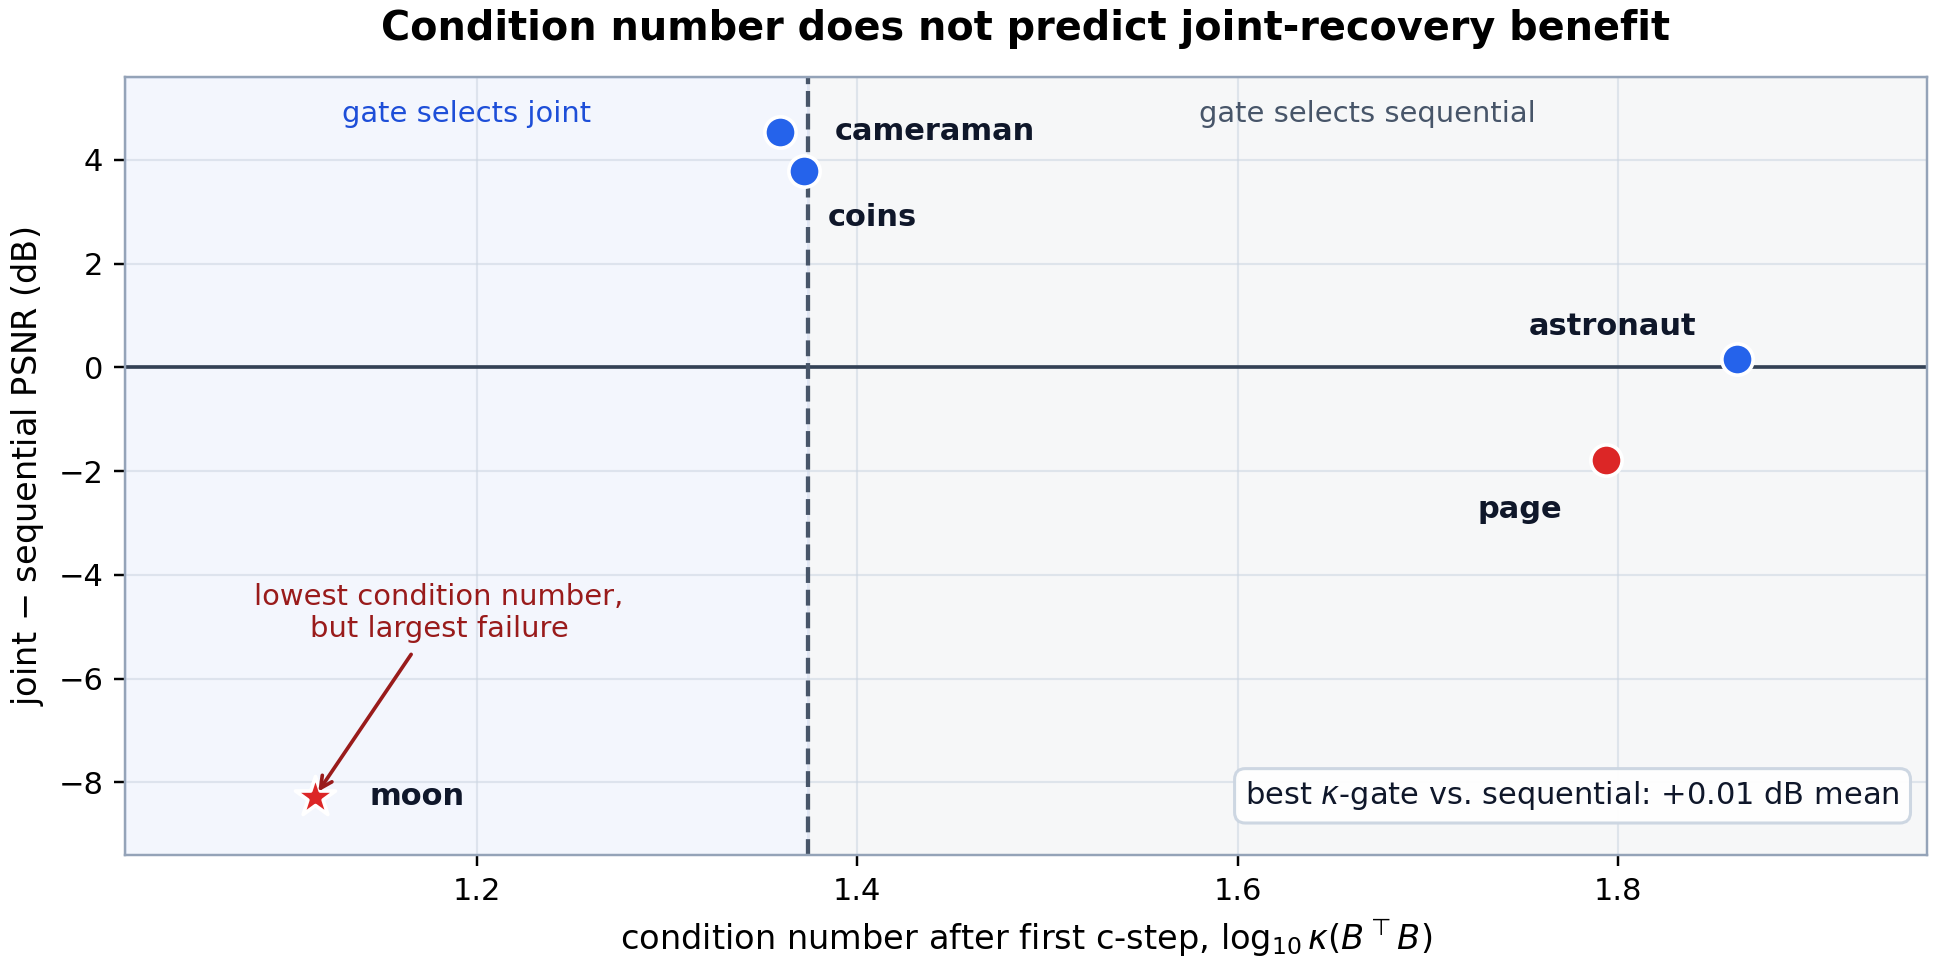
\includegraphics[width=.72\linewidth]{../../figures/identifiability_gate.png}
\caption{Per-scene joint-minus-sequential PSNR.  The best threshold (dashed)
still sends moon---the lowest-$\kappa$ scene and largest loss---to joint.}
\label{fig:gate}
\end{figure}

\paragraph{Falsifying a natural gate.}
At $M/N=0.4$, moon loses $8.27$ dB even though it has the lowest observed
$\log_{10}\kappa(B^\top B)=1.11$; cameraman gains $4.54$ dB at a larger value
of 1.36.  The best threshold sweep improves mean PSNR by only $0.01$ dB over
sequential-only recovery (Figure~\ref{fig:gate}).  Conditioning measures
relative sensitivity, but not the absolute scale of $B$: a low-energy scene
can yield a well-conditioned matrix whose entries are too small relative to
noise.  A useful gate should instead measure a normalized scene-energy or
signal-to-noise statistic after the first coefficient update.  This gate is a
hypothesis for future validation, not a completed result.

\section{Discussion and limitations}

The experiments expose three distinct limits.  First, reducing inner
iterations cannot repair a non-identifiable illumination update.  Second,
training stability is itself an optimization issue: the learned recurrence
can diverge after its best checkpoint as the spectral radius of $W_t$ drifts.
Gradient clipping and best-checkpoint restoration contain the symptom, but a
spectral constraint would be more principled.  Third, the dense representation
dominates asymptotic cost; a ten-layer network is not ``fast'' if every layer
contains a full $N\times N$ map.

The evidence is intentionally limited: five images, synthetic illumination,
Gaussian measurements, one joint patch per scene, five optimizer seeds on one
fixed LISTA operator/dataset, and no modern learned reconstruction baseline.
In particular, we do not call these measurements camera RAW data and do not
claim end-to-end learned joint recovery.  Before a camera-facing claim, the
method needs a real RAW benchmark, structured sensing, operator-distribution
generalization, and comparison with a learned inverse-problem baseline.

\section{Conclusion}

Joint recovery helps textured scenes but fails when scene energy is too low,
a regime conditioning does not detect.  LISTA reduces inner iterations, but
scaling requires structured implicit operators, constrained unfolding, and an
energy-aware fallback.

\clearpage
\bibliography{references}

\end{document}
